%=========================================================================
% (c) Michal Bidlo, Bohuslav K�ena, 2008

\chapter{Introduction}

\chapter{FreeIPA}

FreeIPA (where IPA stands for Identity, Policy and Audit) is an open-source security management solution sponsored by Red Hat aimed primarily at Linux and Unix machines\cite{ipaWeb}.

The project itself combines a number of various existing open-source technologies to achieve the goal of providing centralized authentication and authorization, as well as storing important account information like users or group memberships.
FreeIPA also aims to provide easy management and setup of a domain controller which would otherwise be very difficult by using the same components on your own.

In this chapter I will briefly introduce some of the components FreeIPA uses and describe the architecture of the resulting FreeIPA server solution.

\section{Directory Server}
FreeIPA's directory service is the foundation of the project as it stores various information on behalf of all of FreeIPA's components.
It also plays a big role in authentication and authorization using Kerberos which will be presented in the next section.

The LDAP protocol\cite{ldapRFC} is used as a means of communication with the server and the data itself is stored in a Directory Information Tree (DIT) which is a tree-like data structure.
An example of a DIT structure can be seen in figure \ref{fig:dit}.

\begin{figure}[!ht]
    \centering
        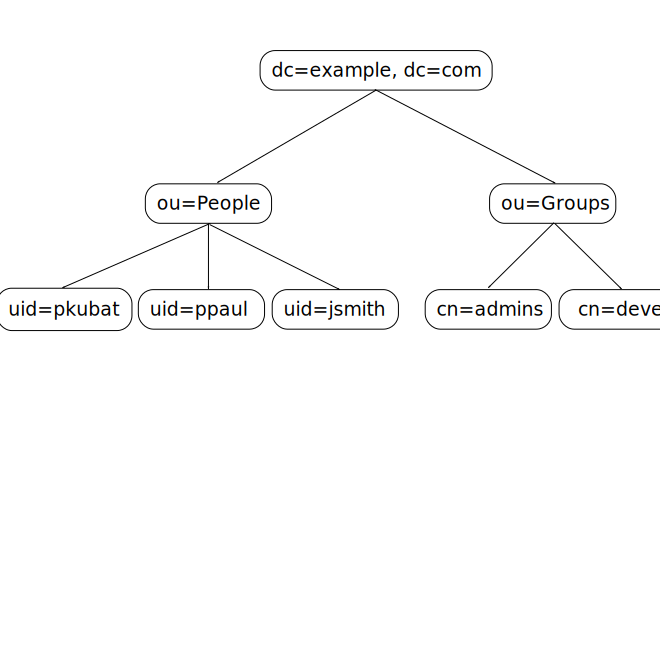
\includegraphics[scale=0.6]{fig/ldap-dit}
    \caption{LDAP Directory Information Tree}
    \label{fig:dit}
\end{figure}

LDAP provides several operations to use with the server\cite{ldapRFC}:

\begin{itemize}
    \item \textbf{add, delete, modify:} These operations add, remove and modify the data contained in the DIT.
    \item \textbf{search, compare:} The search and compare operations are used in querying the DIT for specific information.
    \item \textbf{bind, unbind, abandon:} These operations can be used to authenticate to the directory, terminating the connection or abandoning a previously sent request entirely, respectively.
    \item \textbf{extended operations:} New operations that are not a part of the original protocol.
\end{itemize}

The actual LDAP compatible server contained in FreeIPA is implemented using the 389 Directory Server project\cite{ldapWeb}.
% TODO: ACLs

\section{Kerberos}
Kerberos\cite{kerbRFC} is a network authentication protocol that uses symmetric encryption using a pre-shared key to authenticate the client to a network service (and vice versa) via an insecure connection using a trusted third party service called a Key Distribution Center (KDC). \\
The resulting communication is secure because no secret keys are transported over the network in plaintext format as the KDC already contains a database of credentials for users and services in the Kerberos realm. \\

\begin{figure}[!ht]
    \centering
        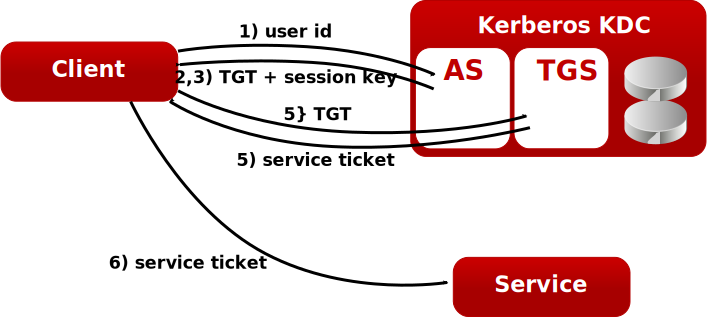
\includegraphics[scale=0.6]{fig/kerb}
    \caption{Kerberos authentication process}
    \label{fig:kerb}
\end{figure}

The process of authenticating the user to a network service is shown in figure \ref{fig:kerb} and can be described in these steps:
\begin{enumerate}
    \item The user sends his principal name (an unique identifier) to the KDC's Authentication Server (AS) via a plaintext request.
    \item The AS then checks the database to make sure the user exists and sends back a randomly generated session key to be used to encrypt communication with another service called a Ticket-Granting Service (TGS) encrypted with the user's secret key.
    \item The AS also generates a set of credentials called a Ticket-Granting Ticket (TGT) which includes the previously generated session key and is encrypted by the secret key of the TGS.
    \item After recieving the first message the client decrypts it using his secret key. This is the only time the user's key is actually used. The TGT which the client can't decrypt himself is saved in a cache on the client's side to be used later to setup a session with the TGS. At this point the user is authenticated to the Kerberos realm and doesn't have to input his secret key again for a set amount of time (commonly 10-24 hours).
    \item When the user wants to authenticate agains a service in the Kerberos realm he just has to ask the TGS to send him a ticket.
    \item The user then authenticates to the chosen service using this ticket without the need for his secret key.
\end{enumerate}

As the security of the Kerberos protocol is partly based on the time stamps of tickets, all of the clients and services in the realm have to be properly synchronized time-wise.
To achieve this goal the Network Time Protocol can be used in the FreeIPA project. \\
FreeIPA's KDC is implemented using the MIT Kerberos\cite{kerbWeb} open source software and FreeIPA also provides its own KDC data backend called ipa-kdb which is used to both read and write user information to FreeIPA's LDAP directory service\cite{kerbIpa}.
\section{DNS}
Even though it would be possible to access network services located in a FreeIPA domain directly using their IP addresses, it is much more easier to do so using domain names. \\
The Domain Name System (DNS)\cite{dnsRFC} is distributed naming system, that translates domain names, which can be easily memorized by humans, into IP addresses using special name servers.
As such if one wants to access a network service or a webpage he doesn't have to remember its IP address, only the IP address of the name server (which is stored localy on the client machine) and the domain name of the service/webpage. \\
The domain name space resembles a tree structure, each node having a label that designates a part of its domain name, while the full domain name of the node can be built by concatenating this label with the domain name of its parent node. \\
The name space is divided into zones starting at the root of the tree structure with child nodes of the root node called top-level domains (TLD).

\begin{figure}[!ht]
    \centering
        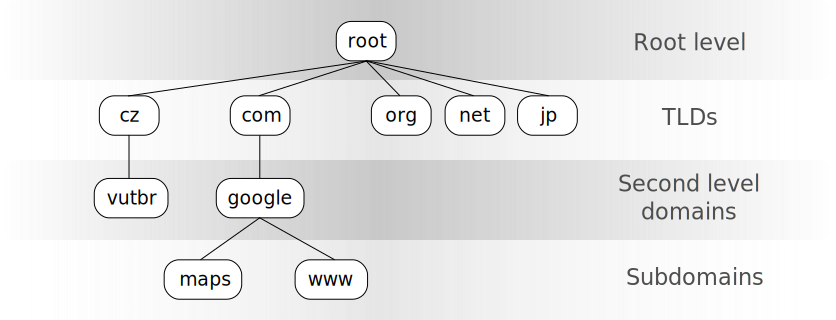
\includegraphics[scale=0.6]{fig/dns-tree}
    \caption{Domain name space}
    \label{fig:dnsTree}
\end{figure}

These zones can contain one or several domains, each domain served by one or several name servers, and can be divided into additional zones if deemed necessary. \\
The DNS server in FreeIPA uses an enhanced BIND name server which allows FreeIPA to store data into an LDAP directory\cite{dnsIpa}.
However using FreeIPA's integrated DNS server is optional and as such the project can be used with a different third party DNS server if so desired.
\section{FreeIPA Architecture}
While the most important components of the FreeIPA project have been described in previous sections, a number of components are still missing for the infrastructure to be complete.

\begin{figure}[!ht]
    \centering
        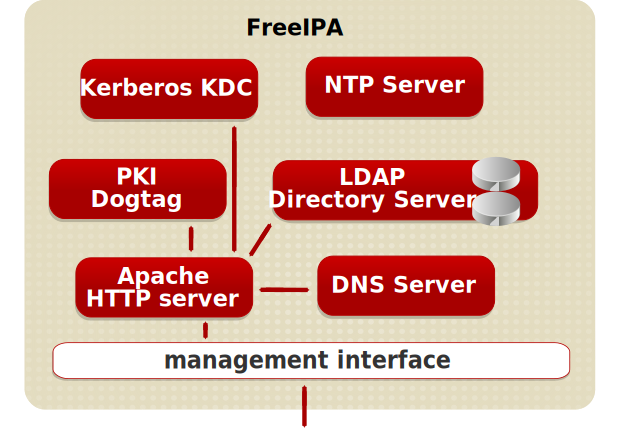
\includegraphics[scale=0.6]{fig/ipa-architecture}
    \caption{High level FreeIPA server architecture}
    \label{fig:ipaHigh}
\end{figure}

To start with, FreeIPA can optionally use the Dogtag project\cite{certWeb} as an integrated Public Key Infrastructure that signs and publishes certificates for hosts and services inside the domain. \\
Secondly, the Apache Web Server is used to provide web based access to the management APIs using the XML-RPC and JSON-RPC APIs as well as to serve the web interface to the clients. \\
And last but not least, as one of the most important additions to the project, FreeIPA's ipalib framework is used together with the Command Line and Web based interfaces to administer the FreeIPA domain. \\
A high level and a detailed representation of the resulting infrastructure can be found in figures \ref{fig:ipaHigh} and \ref{fig:ipaDetail}, respectively.

\begin{figure}[!ht]
    \centering
        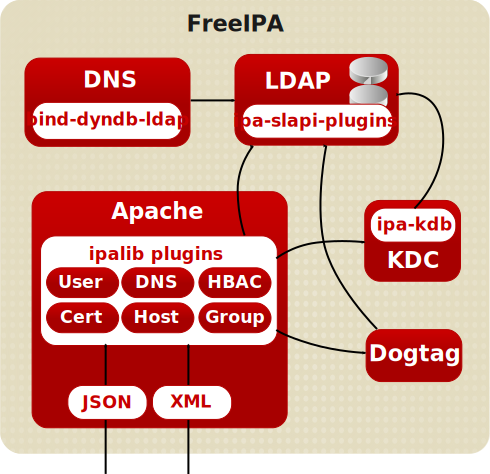
\includegraphics[scale=0.6]{fig/freeipa-detail}
    \caption{Detailed look at FreeIPA architecture}
    \label{fig:ipaDetail}
\end{figure}

The ipalib framework is written using the Python programming language and is highly modular -- most if not all of its functionality is implemented using plug-ins, which are executed on demand using the Apache Server.
This framework is generally used to connect the isolated components into the FreeIPA solution, providing the ability to enroll users or services into the domain, managing the certificates used within the domain or
adding Host Based Access Control rules for even beter access management.

\section{Extending FreeIPA}

\subsection{Extending the Framework}
As previously stated, the ipalib framework is highly modular and extensible with a couple of different ways to add new (or modify current) functionality\cite{extIpa}:\\
First off one can directly extend existing objects of the ipalib framework. These objects are mainly responsible for executing various commands sent using the XML and JSON APIs
and as such extending or modifying the objects, eg. adding a parameter or rewriting an object's label, can alter the default behaviour of those commands. \\
The second way is to extend methods of an object stored in the LDAP database by adding callbacks to these methods.
Callbacks are user-defined functions that are called at various stages of exectution of the method:
\begin{description}
    \item[Pre callback]\hfill \\This callback is called before executing the method's code. Used for modifying arguments and data validation.
    \item[Post callback]\hfill \\This callback is called after executing the method's code and allows for analyzing the result of the command.
    \item[Exc callback]\hfill \\This callback is called in case there is an error during the execution of the method's code. Can be used to recover from the error.
    \item[Interactive callback]\hfill \\Allows a command to decide if additional parameters should be requested from the user.
\end{description}
\subsection{Extending the Directory Server}
The 389 DS used in the FreeIPA project has only one way of creating extensions and that is using server plug-ins.
There are several types of plug-ins that can be used when trying to extend the directory server\cite{extLDAP}:
\begin{description}
    \item[Pre operation]\hfill \\A pre operation plug-in is executed before starting the LDAP operation. Mostly used for data validation.
    \item[Post operation]\hfill \\A post operation plug-in is executed after performing the LDAP operation. Can be used for notifications.
    \item[Entry storage and fetch]\hfill \\Executed before writing and reading data from the database, respectively. An example of this type of plug-in would be encryption/decryption of data saved in the database.
    \item[Extended operation]\hfill \\Executed when the client calls an extended operation.
    \item[Syntax]\hfill \\Run when getting a list of candidates for a search. Can be used to modify comparison operations.
    \item[Matching rule]\hfill \\Run when the client sends a request with an extensible matching search filter.
\end{description}
One can see that there are some similarities to callbacks of ipalib's extensions, especially the way of calling pre and post operations plug-ins is basically the same as pre and post callbacks
differing only in when they are called. While pre and post callbacks are bound to a specific method of a specific command object (eg. before or after executing a user-add command),
the pre and post operations plug-ins are bound to an LDAP operation and as such are run much more frequently.
\chapter{Active Directory}
\chapter{Analyze}
\chapter{Conclusion}

%=========================================================================
